\documentclass[conference,a4paper,10pt]{IEEEtran}
\IEEEoverridecommandlockouts

% Packages
\usepackage[T1]{fontenc}
\usepackage{cite}
\usepackage{amsmath,amssymb,amsfonts}
\usepackage{mathptmx}              % Times text + math, IEEE-canonical
\usepackage{algorithmic}
\usepackage{graphicx}
\usepackage{textcomp}
\usepackage{xcolor}
\usepackage{booktabs}
\usepackage{tabularx}
\usepackage{multirow}
\usepackage{microtype}
\usepackage[hidelinks,colorlinks=false]{hyperref}
\usepackage{caption}
\captionsetup{font=footnotesize,labelfont={bf,sf}}

\def\BibTeX{{\rm B\kern-.05em{\sc i\kern-.025em b}\kern-.08em
    T\kern-.1667em\lower.7ex\hbox{E}\kern-.125emX}}

\graphicspath{{figures_ieee/}}

\hypersetup{
    pdfauthor={Gursahib Singh and Deeparsh Singh Dang},
    pdftitle={Which RAG for Which Domain? An Open Framework for Comparative Evaluation},
}

\begin{document}

\title{Which RAG for Which Domain?\\
{\Large An Open, Model-Agnostic Framework for\\Comparative Evaluation of Retrieval-Augmented Generation Strategies}\\
\thanks{This work is released as an open-source research framework. The complete codebase (reference approach implementations, evaluation harness, statistical tooling, interactive studio, and reproducibility scripts) is publicly available at \url{https://github.com/Singh-Gursahib/RAG-Approaches} for community use, extension, and contribution. The framework is intentionally model-agnostic: practitioners are encouraged to plug in their own datasets, swap in alternative generators or retrievers, and reuse the per-call cost ledger to characterize their specific deployment.}}

\author{
\IEEEauthorblockN{Gursahib Singh$^{1}$ and Deeparsh Singh Dang$^{2}$}
\IEEEauthorblockA{Thompson Rivers University\\
$^{1}$gursahib99888@gmail.com \hspace{1cm} $^{2}$deeparshsingh10@gmail.com}
}

\maketitle

\begin{abstract}
The Retrieval-Augmented Generation (RAG) literature~\cite{lewis2020rag} offers many architectural variants, from naive vector retrieval and hybrid lexical and dense fusion to hypothetical-document embeddings, cross-encoder reranking, and graph-based, hierarchical, and self-reflective retrieval. Yet practitioners choosing an approach for a specific domain rarely see a head-to-head comparison run under matched conditions on data resembling their own.
We address this gap with an open, model-agnostic framework for comparative RAG evaluation that any researcher or practitioner can customize and extend.
It provides reference implementations of seven approaches (four RAG variants and three non-retrieval long-context strategies), a probe-type taxonomy that separates honesty, single-fact recall, multi-hop reasoning, and distractor robustness, percentile-bootstrap confidence intervals~\cite{efron1979bootstrap} with Holm-corrected paired Wilcoxon tests~\cite{wilcoxon1945,holm1979}, a per-call cost ledger, and an interactive studio that runs the evaluation on any hosted model.
As a case study we evaluate a hand-authored 8K-token corpus with 34 questions on two generators, the proprietary Gemini~3~Flash~\cite{gemini2024} and the open-weights GLM~5.3~Flash, each with three seeds.
Four findings emerge.
First, the four retrieval pipelines transfer across generators: their F$_1$ scores differ by at most 3.8 points between the two models, while F$_1$ spans up to 67.5 points across strategies on a single model, so the choice of pipeline matters far more than the choice between these generators.
Second, Full-Context is the strongest strategy on both generators (F$_1$ $0.881$ and $0.915$), provided a reasoning model is given enough token headroom; without it, GLM~5.3~Flash falls to $0.490$.
Third, question-agnostic summarization loses specific facts on both generators, but the size of its overall deficit depends on the model (F$_1$ $0.206$ against $0.717$).
Fourth, a strict refusal prompt yields perfect refusal accuracy for every retrieval strategy on both generators.
We translate these probe-level results into domain-aware recommendations for medical, legal, educational, code, and finance use cases.
The framework's central deliverable is not these specific numbers but the ability for any reader to reproduce and extend this evaluation on their own domain and model at low cost.
\end{abstract}

\begin{IEEEkeywords}
Retrieval-Augmented Generation, model-agnostic evaluation framework, cross-model replication, domain-specific RAG, reasoning language models, long-context language models, reproducible NLP.
\end{IEEEkeywords}

\section{Introduction}
\label{sec:intro}

Retrieval-Augmented Generation (RAG)~\cite{lewis2020rag,karpukhin2020dpr} has become the dominant architectural pattern for grounding Large Language Models (LLMs) in private or domain-specific corpora.
Within five years the technique has expanded from a single recipe into a sprawling family of variants, including HyDE~\cite{gao2023hyde}, GraphRAG~\cite{edge2024graphrag}, RAPTOR~\cite{sarthi2024raptor}, Self-RAG~\cite{asai2024selfrag}, hybrid retrieval~\cite{cormack2009rrf}, and cross-encoder reranking~\cite{khattab2020colbert,xiao2023cpack}, each targeting a specific failure mode of its predecessor.
At the same time, the assumption that motivated RAG in the first place, that the documents will not fit in the model's context window, is rapidly weakening~\cite{gemini2024}. Whether retrieval still earns its complexity at modern context scales is therefore an empirical question.

For a practitioner choosing a RAG strategy for a specific domain, this profusion is unhelpful.
A medical question-answering system has different requirements than a legal-citation retrieval system or an educational tutor: needle-style recall is critical when answers depend on specific drug names or statute numbers, multi-hop reasoning matters when conclusions chain across documents, and refusal honesty is essential whenever a wrong answer is worse than no answer.
Yet the published literature largely reports each new RAG variant in isolation, on benchmarks chosen to highlight its strengths, often against a different baseline configuration than the next paper.
A head-to-head comparison under matched conditions (same generator, same chunker, same evaluation protocol, same probe taxonomy) on data that resembles the practitioner's deployment is rare, and building one from scratch typically takes weeks of engineering.

A second question is how much such a comparison depends on the generator.
If the relative performance of RAG strategies changed with every model, a comparison would have to be repeated for each one.
If the pipelines transfer, the choice of pipeline can be made once for a given corpus and question mix, and revisited only when those change.

\subsection{Our contribution: a framework, not a verdict}

This paper makes a software-engineering contribution as well as an empirical one.
Our primary deliverable is an open-source framework, designed to be reused, customized, and extended by anyone evaluating RAG strategies for a specific use case.
The framework provides:

\begin{itemize}
    \item \textbf{Reference implementations} of four RAG variants (Naive, Hybrid, HyDE, Cross-Encoder Reranker) and three non-retrieval strategies (Full-Context Injection, Recursive Summarization, Sliding-Window Reasoning), all behind a common \texttt{Approach} protocol that takes a single configuration object and emits a uniform per-question prediction record.
    \item \textbf{A probe-type evaluation taxonomy} (sanity, hallucination, needle, multi-hop, distractor) that lets a domain practitioner compose an evaluation set whose mix of probe types reflects the questions their users actually ask.
    \item \textbf{Statistical infrastructure}: percentile-bootstrap 95\% confidence intervals~\cite{efron1979bootstrap}, paired Wilcoxon signed-rank tests~\cite{wilcoxon1945}, and Holm-corrected~\cite{holm1979} multiple-comparison adjustment, all callable from a single command-line entry point.
    \item \textbf{A model-agnostic generation layer}, demonstrated here with two backends: a direct Gemini client used for the original sweep, and an OpenRouter client that reaches hosted proprietary and open-weights models through one OpenAI-compatible interface. Changing the generator is a configuration change; the chunker, retrievers, evaluator, statistics, and ledger are untouched.
    \item \textbf{A per-call cost ledger} that records the cost of every model call, so practitioners can characterize the financial cost of any approach against any model on their own data.
    \item \textbf{RAG Atlas}, an interactive studio that runs the same reference implementations live on user documents with any OpenRouter model, repeats evaluations across seeds, saves every finished test, and can replay this paper's case study on a new model.
\end{itemize}

The framework's central premise is that the comparative evaluation reported in Section~\ref{sec:results} should be replicable on \emph{any} domain by anyone, in roughly an hour, on a personal laptop, with whichever LLM they prefer.
The specific numbers we report for a synthetic 8K-token corpus are an illustrative case study; the per-domain recommendations in Section~\ref{sec:domain} are a starting point that we expect users of the framework to refine on their own data.

\subsection{Case-study findings}

To demonstrate the framework and to seed domain-aware recommendations, we run all seven reference approaches on a hand-authored 34-question evaluation set spanning five probe types, with three random seeds per approach at temperature~$0.3$, on two generators: Gemini~3~Flash and the open-weights GLM~5.3~Flash.
Four findings, in brief:

\begin{enumerate}
    \item \textbf{Pipelines transfer across generators.} Each of the four retrieval strategies scores within 3.8 F$_1$ points of its own result on the other model, and every GLM~5.3~Flash estimate for these strategies lies inside the corresponding Gemini~3~Flash confidence interval. On a single model, by contrast, F$_1$ varies by up to 67.5 points across strategies. For these generators, which pipeline is used matters far more than which model runs it.
    \item \textbf{Full-Context leads on both generators, given reasoning headroom.} At sub-window corpus scale ($\approx 8{,}000$ tokens), placing the corpus in the prompt gives the highest F$_1$ on Gemini~3~Flash ($0.881$) and on GLM~5.3~Flash ($0.915$). GLM~5.3~Flash always reasons, and with a 640-token limit its reasoning ran out of room on the long prompt, cutting F$_1$ to $0.490$.
    \item \textbf{Summarization loss is model-dependent in size.} Question-agnostic recursive summarization drops the identifiers and numbers that factoid questions ask about on both generators (needle-probe F$_1$ $0.00$ and $0.31$), but its overall F$_1$ ranges from $0.206$ to $0.717$ depending on the model.
    \item \textbf{Prompt-level honesty transfers for retrieval pipelines.} The strict-refusal prompt (``if the context does not contain enough information, respond with NOT\_IN\_CONTEXT'') achieves perfect refusal accuracy for all four retrieval strategies on both generators; a multi-step non-retrieval pipeline lost some of that honesty on GLM~5.3~Flash.
\end{enumerate}

The remainder of the paper proceeds as follows.
Section~\ref{sec:related} surveys retrieval, long-context, and domain-specific RAG literature.
Section~\ref{sec:framework} describes the framework's design principles and extension points.
Section~\ref{sec:methods} specifies the seven reference approaches.
Section~\ref{sec:setup} describes the case-study corpus, probe taxonomy, metrics, and generators.
Section~\ref{sec:results} reports results on both generators.
Section~\ref{sec:domain} synthesizes probe-type findings with the domain-specific RAG literature to provide per-domain guidance.
Section~\ref{sec:discussion} discusses the broader takeaways, Section~\ref{sec:limits} catalogs explicit extension points, and Section~\ref{sec:conclusion} concludes.

\section{Related Work}
\label{sec:related}

\subsection{Retrieval-Augmented Generation}
RAG~\cite{lewis2020rag} couples a parametric language model with a non-parametric document store, retrieved at inference time via a dense passage retriever~\cite{karpukhin2020dpr}.
Dense retrievers are typically trained as sentence encoders, with Sentence-BERT~\cite{reimers2019sbert} introducing the siamese fine-tuning recipe that the \texttt{sentence-transformers} ecosystem (and our framework's default embedding model, \texttt{all-MiniLM-L6-v2}) inherits.

Two improvement axes are widely studied.
First, retrieval quality can be enhanced by combining lexical~\cite{robertson2009bm25} and dense signals via Reciprocal Rank Fusion~\cite{cormack2009rrf} or by adding a cross-encoder reranker~\cite{khattab2020colbert,xiao2023cpack} that scores query-document pairs jointly.
Second, query reformulation methods such as HyDE~\cite{gao2023hyde} sidestep the surface-form gap between question and answer text by first generating a hypothetical answer and embedding \emph{that}.

A separate line of work builds structured retrieval indices.
GraphRAG~\cite{edge2024graphrag} extracts an entity-and-relation graph and pre-computes community-level summaries; RAPTOR~\cite{sarthi2024raptor} builds a recursive summarization tree.
Self-RAG~\cite{asai2024selfrag} introduces reflection tokens that let the model decide on demand whether to retrieve at all.
These structured and adaptive approaches are first-class targets for inclusion in the framework as community contributions; we discuss the extension protocol in Section~\ref{sec:framework}.

\subsection{Long-Context Models and the End of RAG?}
Modern frontier flash-tier models~\cite{gemini2024} accept on the order of $10^6$ input tokens, raising the question of whether retrieval continues to earn its complexity once the corpus fits.
Liu et al.~\cite{liu2024lostmiddle} report a U-shaped accuracy curve with respect to evidence position in the prompt, the ``lost in the middle'' phenomenon, suggesting that simply concatenating a long corpus is not free of failure modes.
Many current flash-tier models also reason before answering, which adds a second budget, the tokens spent thinking, that interacts with long prompts (Section~\ref{sec:headroom}).
Our framework measures these trade-offs directly on whatever corpus and model the user supplies.

\subsection{Domain-Specific RAG Evaluation}
Most directly relevant to our domain-aware framing, MedRAG~\cite{xiong2024medrag} benchmarks RAG configurations against the MIRAGE suite of 7{,}663 medical QA items across five datasets, characterizing how retriever choice interacts with model scale.
LegalBench~\cite{guha2023legalbench} provides 162 legal-reasoning tasks contributed by legal professionals; LegalBench-RAG~\cite{pipitone2024legalbenchrag} extends the benchmark to evaluate retrieval mechanisms specifically.
Both efforts demonstrate that the same RAG variant can rank very differently across domains, motivating our framework's emphasis on user-supplied corpora and per-domain replication rather than a single universal verdict.

\subsection{Evaluation Methodology}
Our metrics follow the SQuAD~\cite{rajpurkar2016squad} normalization conventions for token-level Exact Match and $F_1$.
Multi-hop probe design is informed by HotpotQA~\cite{yang2018hotpot}.
For statistical inference we use the percentile bootstrap~\cite{efron1979bootstrap}, the paired Wilcoxon signed-rank test~\cite{wilcoxon1945}, and Holm's sequentially rejective correction~\cite{holm1979} to bound the family-wise error rate across pairwise tests.

\section{Framework Design}
\label{sec:framework}

The framework is built around four explicit design principles, each intended to make the empirical study below repeatable on data and models the framework's authors have never seen.

\paragraph{P1.~Model-agnostic generation.}
All generation flows through a thin client interface centered on a single \texttt{generate} call that returns the answer text with its token counts, cost, and latency.
The original sweep uses a Gemini implementation~\cite{gemini2024} configured via the \texttt{GOOGLE\_API\_KEY} environment variable.
The replication uses an OpenRouter implementation that reaches hosted proprietary and open-weights models through one OpenAI-compatible API, records the cost reported for every call, and sets the reasoning effort of models that reason before answering.
It sends no application-identifying headers, so evaluation traffic is not attributed to the framework.
Other providers, including locally hosted models, need only the same call and a per-token price for the cost ledger.

\paragraph{P2.~Approach-pluggable retrieval.}
Each reference approach implements a common \texttt{Approach} protocol whose entry point, \texttt{answer(question, corpus, llm)}, is the only contract a new approach must satisfy.
A contributor who wishes to add, say, a GraphRAG~\cite{edge2024graphrag} or RAPTOR~\cite{sarthi2024raptor} implementation does so by writing a single Python class and registering it; the evaluator, ledger, statistical tests, and studio all pick up the new approach without modification.
The seven approaches in this paper are reference implementations, not the framework's final inventory.

\paragraph{P3.~Domain-pluggable evaluation.}
The evaluator consumes two inputs: a corpus directory and a JSONL file of question records, each carrying \texttt{(qid, type, question, gold\_answer, source\_doc, source\_span)}.
The five probe types we use (sanity, hallucination, needle, multi-hop, distractor) are recommendations, not requirements; users may add new probe types or remove unused ones with no code changes.
The probe-type breakdown then propagates automatically into the headline table, the per-probe heatmap, and the cost analysis.

\paragraph{P4.~Cost transparency.}
Every model call writes one JSONL row containing timestamp, approach, probe id, prompt tokens, completion tokens, dollar cost, and wall-clock latency.
For hosted gateways the ledger records the cost the provider reports; otherwise cost is computed from token counts and a price table.
A configurable hard cap (default \$5) refuses to launch any call that would push cumulative spend above 95\% of the cap.
The ledger lets a practitioner reproduce the cost calculations in this paper for an arbitrary alternative model, or set a much smaller cap for a personal exploration.

\paragraph{Interactive studio.}
RAG Atlas wraps the unchanged reference implementations, metrics, and statistics in a web application.
Users load documents, choose strategies and a generator, and inspect each retrieval and generation step with its tokens, latency, and cost as every strategy completes.
An evaluation mode grades a user's own question set; a replay mode reruns this paper's corpus and questions on any model with the paper's settings and places the results beside the published ones.
Finished tests are saved and can be reopened without re-running.
The GLM~5.3~Flash replication in Section~\ref{sec:crossmodel} was produced this way.

\paragraph{Extensibility, not restriction.}
Each numeric parameter in the case study is exposed as a configuration field rather than a hard-coded constant: the 150-token chunk window, the top-$k$ of~5, the reranker's top-$n$ of~20, the temperature of~$0.3$, the answer budget of 512 tokens, the eval-set size of~34, the seed count of~3, the corpus size of $\approx 8{,}000$ tokens, and the \$5 budget cap.
A practitioner with a different domain, a larger corpus, or a different cost envelope is expected to override these defaults; the values we use are reference settings chosen to let the case study reproduce in about an hour for about a dollar, not normative claims about how RAG should be deployed.

\section{Reference Approaches}
\label{sec:methods}

We provide reference implementations of seven approaches.
Sections~\ref{sec:rag-methods} and~\ref{sec:nonrag-methods} describe their pipelines; Fig.~\ref{fig:pipelines} provides a visual side-by-side.
A common answer-generation prompt is used across every retrieval-style approach: the model is asked to answer using only the provided context and, when no answer is grounded, to emit the sentinel \texttt{NOT\_IN\_CONTEXT}.
Identical chunking (sentence-window, target~150 tokens, 30-token overlap) is used across every retrieval approach in the case study, but all of these defaults are configuration-overridable per Section~\ref{sec:framework}.

\begin{figure*}[!t]
\centering
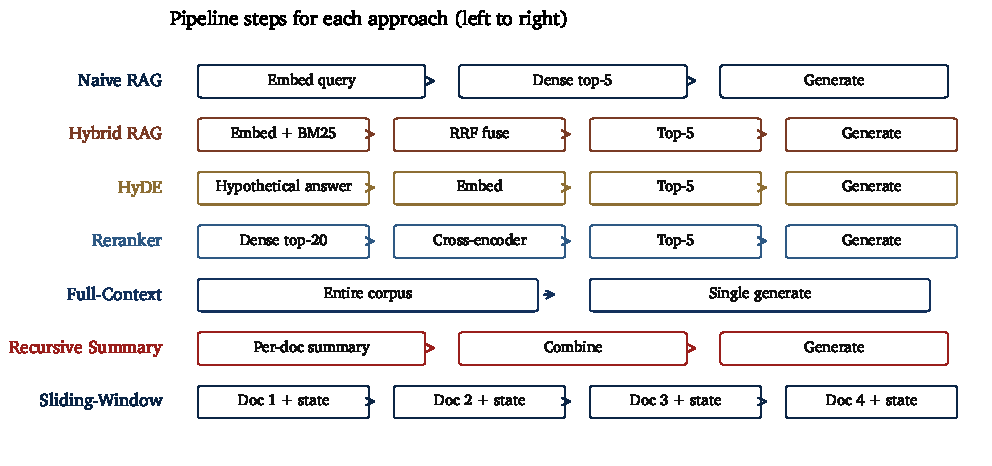
\includegraphics[width=0.95\textwidth]{pipelines.pdf}
\caption{Stepwise structure of the seven reference approaches. Each row is one of the framework's seven plug-in implementations; the \texttt{Approach} protocol is the contract a contributor satisfies to add an eighth. Single-call approaches occupy the upper rows; multi-call approaches occupy the lower rows.}
\label{fig:pipelines}
\end{figure*}

\subsection{Retrieval-Style Approaches}
\label{sec:rag-methods}

\paragraph{Naive Vector RAG (R1).}
The minimal RAG baseline.
The query is embedded with \texttt{all-MiniLM-L6-v2}~\cite{reimers2019sbert}; the top five chunks under cosine similarity in a ChromaDB index are spliced into the prompt; one generation call produces the answer.
This is the floor against which every other RAG variant in the framework must justify its additional complexity.

\paragraph{Hybrid RAG (R2).}
Dense top-$N$ and BM25~\cite{robertson2009bm25} top-$N$ rankings are fused via Reciprocal Rank Fusion (RRF)~\cite{cormack2009rrf}.
For a chunk $c$ appearing at rank $r_i(c)$ in retriever $i$, its fused score is
\begin{equation}
\mathrm{RRF}(c) = \sum_{i \in \{\mathrm{dense},\mathrm{BM25}\}} \frac{1}{k + r_i(c)}, \quad k = 60,
\label{eq:rrf}
\end{equation}
with $k$ set per the empirical recommendation of~\cite{cormack2009rrf}.
The top-5 fused chunks are passed to generation.

\paragraph{HyDE (R3).}
The generator first writes a confident hypothetical answer to the question; that hypothetical is embedded; the top-5 chunks closest to the hypothetical's embedding are retrieved~\cite{gao2023hyde}.
The final answer generation runs over those chunks with the standard answer prompt.
HyDE costs two LLM invocations per question.

\paragraph{Cross-Encoder Reranker (R4).}
A wider dense top-$N=20$ candidate set is rescored by a cross-encoder (\texttt{bge-reranker-base}~\cite{xiao2023cpack}) that takes the query-document pair as joint input.
The top-5 after reranking are used.
The reranker runs locally; the only cloud cost is the single subsequent generation call.

\subsection{Non-Retrieval Approaches}
\label{sec:nonrag-methods}

\paragraph{Full-Context Injection (N1).}
The entire corpus is concatenated and placed in the prompt verbatim; a single generation call produces the answer.
Cost scales linearly in corpus tokens.

\paragraph{Recursive Map-Reduce Summarization (N2).}
A one-time setup step summarizes each document with an explicit ``preserve all specific facts'' instruction.
The concatenated summaries form the answer-time context.

\paragraph{Sliding-Window Reasoning (N3).}
The corpus is processed one document at a time with a running ``best answer state.''
Four documents yield four generation calls per question, in series with state carry-over.

\section{Case Study: Experimental Setup}
\label{sec:setup}

The following experiment is one illustration of how the framework is used; the framework itself supports any corpus and any LLM backend.

\subsection{Corpus}
\label{sec:corpus}

We author a four-document fictional corpus totaling 5{,}983 words ($\approx 8{,}000$ tokens) describing (i)~the \emph{Halden Institute for Computational Mycology}, (ii)~the \emph{City of Veridian}, (iii)~the \emph{MERIDIAN-7 Satellite System}, and (iv)~the \emph{Auralite Accord of 1987}, with deliberate cross-references between documents that enable genuine multi-hop probes.

A hand-authored corpus has three properties not easily obtained from public benchmarks.
First, every gold answer is verifiably grounded.
Second, distinctive identifiers (e.g., \texttt{MULBERRY-7Q}, \texttt{4.832~GHz}) can be planted at controlled depths to test long-tail recall.
Third, hallucination probes can be constructed with confidence that their answer is \emph{absent} from the corpus.
None of these properties is required by the framework; users with a domain corpus simply supply their own.

\subsection{Probe Taxonomy}
\label{sec:probes}

The evaluation set contains 34 questions partitioned across five probe types: \textbf{Sanity (4)}, \textbf{Needle-in-haystack (8)}, \textbf{Multi-hop (8)}, \textbf{Distractor (8)}, and \textbf{Hallucination (6)}.
The 34-question total is a case-study size, chosen to let the experiment reproduce inexpensively; the framework supports evaluation sets of arbitrary size, and we expect domain practitioners to use substantially larger sets when the marginal cost of evaluation is acceptable.

\subsection{Metrics}
\label{sec:metrics}
Token-level Exact Match (EM) and $F_1$ follow the SQuAD normalization~\cite{rajpurkar2016squad}: lowercase, strip punctuation and articles, collapse whitespace; identifier hyphens are replaced with spaces so that, e.g., \texttt{MULBERRY-7Q} and \texttt{MULBERRY 7Q} normalize identically.
For hallucination probes, a prediction counts as correct if and only if it matches one of a curated set of refusal phrases.
Per-approach metrics are reported with percentile-bootstrap 95\% CIs~\cite{efron1979bootstrap} computed over $B = 2000$ resamples.

\subsection{Statistical Tests}
\label{sec:stats}
Pairwise approach comparisons use the paired Wilcoxon signed-rank test~\cite{wilcoxon1945} on the per-question grade differences; raw $p$-values are Holm-corrected~\cite{holm1979} across all $\binom{7}{2}=21$ pairs.

\subsection{Generators, Seeds, and Budget}
\label{sec:execution}
Both generators run under identical retrieval and evaluation settings: \texttt{all-MiniLM-L6-v2}~\cite{reimers2019sbert} embeddings, a \texttt{bge-reranker-base}~\cite{xiao2023cpack} cross-encoder, ChromaDB and \texttt{rank\_bm25} indexes, the same prompts and grading, a 512-token answer budget, temperature~$0.3$, and three seeds per approach.

\emph{Gemini~3~Flash} (\texttt{gemini-3-flash-preview}~\cite{gemini2024}) is the original sweep, called directly through Google's API under a hard \$5 spending cap; it consumed \$1.09.
Its per-run costs are ledger estimates computed from token counts at \$0.30 and \$2.50 per million input and output tokens.

\emph{GLM~5.3~Flash} (\texttt{z-ai/glm-5.3-flash}, with open weights published as \texttt{zai-org/GLM-5.3-Flash}) is the replication, run through the studio's replay mode via OpenRouter.
The model always reasons before answering.
The main run requested low reasoning effort with a 640-token limit, which reserves 20\% of the limit for reasoning.
A Full-Context follow-up used high effort with a 2{,}560-token limit, preserving the same 512 tokens for the answer (Section~\ref{sec:headroom}).
Its costs are the amounts OpenRouter reported for each call.
The replication, the follow-up, and a single-run check together cost \$0.26.

\emph{None of these choices is structural to the framework}: a researcher with a larger budget, a different model, a different embedding, or a different seed count overrides each through configuration.

\section{Case-Study Results}
\label{sec:results}

\subsection{Headline Performance on Gemini~3~Flash}
\label{sec:headline}

Table~\ref{tab:headline} reports the original Gemini~3~Flash sweep with pooled bootstrap 95\% confidence intervals.

\begin{table*}[!t]
\centering
\caption{Case-study headline metrics on Gemini~3~Flash across all seven reference approaches. Mean across three random seeds at $T = 0.3$; uncertainty is the standard deviation across seeds. The $F_1$ CI column gives bootstrap-pooled 95\% confidence intervals across all $34 \cdot 3 = 102$ question-seed grades. Cost is the estimated mean USD per full eval-set run; the entire sweep used 1.09~USD.}
\label{tab:headline}
\renewcommand{\arraystretch}{1.15}
\begin{tabular}{l c c c c c c c}
\toprule
\textbf{Approach} & \textbf{Family} & \textbf{EM} ($\mu \pm \sigma$) & $\boldsymbol{F_1}$ ($\boldsymbol{\mu \pm \sigma}$) & $\boldsymbol{F_1}$ \textbf{95\% CI} & \textbf{Cost (USD)} & \textbf{$p_{50}$ latency (ms)} & \textbf{$p_{95}$ latency (ms)}\\
\midrule
Full-Context        & non-RAG & $0.667 \pm 0.017$ & $\mathbf{0.881 \pm 0.012}$ & $[0.840, 0.918]$ & $0.0912$ & $\phantom{0}18{,}866$ & $\phantom{0}65{,}349$\\
Sliding-Window      & non-RAG & $\mathbf{0.696 \pm 0.045}$ & $0.875 \pm 0.025$ & $[0.826, 0.920]$ & $0.0972$ & $\phantom{00}8{,}317$ & $\phantom{0}10{,}643$\\
HyDE                & RAG     & $0.667 \pm 0.017$ & $0.838 \pm 0.012$ & $[0.780, 0.893]$ & $0.0186$ & $\phantom{00}4{,}999$ & $\phantom{00}7{,}370$\\
Naive RAG           & RAG     & $0.667 \pm 0.017$ & $0.836 \pm 0.012$ & $[0.778, 0.888]$ & $0.0122$ & $\phantom{00}2{,}532$ & $\phantom{00}7{,}937$\\
Reranker            & RAG     & $0.667 \pm 0.017$ & $0.833 \pm 0.009$ & $[0.774, 0.887]$ & $0.0123$ & $\phantom{00}2{,}756$ & $\phantom{00}3{,}786$\\
Hybrid RAG          & RAG     & $0.627 \pm 0.017$ & $0.797 \pm 0.010$ & $[0.728, 0.857]$ & $0.0122$ & $\phantom{00}2{,}058$ & $\phantom{00}7{,}813$\\
Recursive Summary   & non-RAG & $0.206 \pm 0.000$ & $0.206 \pm 0.000$ & $[0.128, 0.284]$ & $0.0068$ & $\phantom{00}3{,}179$ & $\phantom{0}12{,}746$\\
\bottomrule
\end{tabular}
\end{table*}

The two non-retrieval approaches occupy the top: Full-Context ($F_1 = 0.881$) and Sliding-Window ($F_1 = 0.875$) outperform every RAG variant.
Among the RAG family, HyDE, Naive, and Reranker cluster tightly at $F_1 \in [0.833, 0.838]$; Hybrid trails at $0.797$ and Recursive Summary is a clear outlier at $0.206$.
With the single exception of Sliding-Window ($\mathrm{EM}=0.696$), EM clusters at $0.667 \pm 0.017$ across six approaches, a formatting ceiling discussed in Section~\ref{sec:discussion} rather than a retrieval limitation.

\subsection{Pairwise Significance}
\label{sec:significance}

On Gemini~3~Flash, Holm-corrected pairwise Wilcoxon tests identify only one significantly different approach: Recursive Summary, with $p_{\mathrm{adj}} \leq 3 \times 10^{-3}$ against every other approach.
All other pairwise tests yield $p_{\mathrm{adj}} = 1.000$.
On GLM~5.3~Flash, the low-headroom Full-Context run differs significantly from all six other approaches ($p_{\mathrm{adj}} \leq 4 \times 10^{-4}$), and Recursive Summary differs from Reranker ($p_{\mathrm{adj}} = 0.014$); no two retrieval strategies are separable.
At $N = 34$ the statistical power is insufficient to order the retrieval strategies on either generator, and the framework makes it straightforward to run larger evaluations on a user's own corpus to resolve such distinctions.

\subsection{Cross-Model Replication on GLM~5.3~Flash}
\label{sec:crossmodel}

\begin{table*}[!t]
\centering
\caption{Cross-model replication. Token $F_1$ on Gemini~3~Flash (Table~\ref{tab:headline}) and GLM~5.3~Flash for the same corpus, questions, prompts, and grading, with three seeds at $T=0.3$ on both. GLM~5.3~Flash used low reasoning effort with a 640-token limit; the last row repeats Full-Context with high effort and a 2{,}560-token limit (Section~\ref{sec:headroom}). GLM costs are amounts billed by OpenRouter, whereas Gemini costs are ledger estimates, so costs compare only approximately. Latency is the median per run.}
\label{tab:crossmodel}
\renewcommand{\arraystretch}{1.15}
\setlength{\tabcolsep}{4.5pt}
\begin{tabular}{l c c c c c c c}
\toprule
\textbf{Approach} & \textbf{Gemini} $\boldsymbol{F_1}$ & \textbf{GLM} $\boldsymbol{F_1}$ & \textbf{GLM} $\boldsymbol{F_1}$ \textbf{95\% CI} & $\boldsymbol{\Delta F_1}$ & \textbf{GLM EM} & \textbf{GLM cost (USD)} & \textbf{GLM} $\boldsymbol{p_{50}}$ \textbf{(ms)}\\
\midrule
Full-Context        & $0.881 \pm 0.012$ & $0.490 \pm 0.038$ & $[0.405, 0.573]$ & $-0.391$ & $0.363$ & $0.0094$ & $6{,}264$\\
Sliding-Window      & $0.875 \pm 0.025$ & $0.808 \pm 0.041$ & $[0.743, 0.868]$ & $-0.066$ & $0.647$ & $0.0348$ & $3{,}026$\\
HyDE                & $0.838 \pm 0.012$ & $0.813 \pm 0.017$ & $[0.744, 0.875]$ & $-0.025$ & $0.657$ & $0.0073$ & $2{,}491$\\
Naive RAG           & $0.836 \pm 0.012$ & $0.862 \pm 0.000$ & $[0.806, 0.911]$ & $+0.026$ & $0.706$ & $0.0042$ & $697$\\
Reranker            & $0.833 \pm 0.009$ & $0.871 \pm 0.007$ & $[0.823, 0.917]$ & $+0.038$ & $0.696$ & $0.0051$ & $1{,}355$\\
Hybrid RAG          & $0.797 \pm 0.010$ & $0.833 \pm 0.000$ & $[0.768, 0.889]$ & $+0.036$ & $0.676$ & $0.0043$ & $629$\\
Recursive Summary   & $0.206 \pm 0.000$ & $0.717 \pm 0.044$ & $[0.631, 0.792]$ & $+0.511$ & $0.598$ & $0.0109$ & $765$\\
\midrule
Full-Context, headroom & $0.881 \pm 0.012$ & $\mathbf{0.915 \pm 0.007}$ & $[0.880, 0.947]$ & $+0.034$ & $0.755$ & $0.0070$ & $1{,}106$\\
\bottomrule
\end{tabular}
\end{table*}

\begin{figure}[!t]
\centering
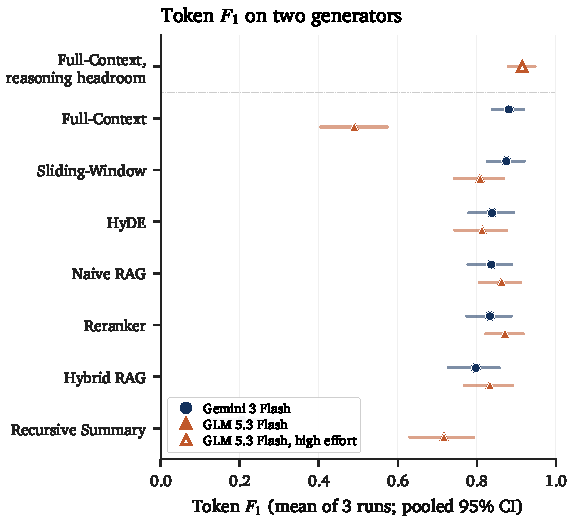
\includegraphics[width=0.95\columnwidth]{cross_model_f1.pdf}
\caption{Token $F_1$ for each strategy on both generators, with pooled bootstrap 95\% CIs over 102 question-seed grades. The four retrieval strategies overlap almost completely across models. The top row shows GLM~5.3~Flash on Full-Context once its reasoning has room (Section~\ref{sec:headroom}).}
\label{fig:crossf1}
\end{figure}

Table~\ref{tab:crossmodel} and Fig.~\ref{fig:crossf1} replicate the case study on GLM~5.3~Flash.
The central result concerns the four retrieval strategies.
Their $F_1$ differs between the two generators by at most $3.8$ points (mean $3.1$), GLM~5.3~Flash is slightly ahead on Naive, Hybrid, and Reranker and slightly behind on HyDE, and every GLM estimate lies inside the corresponding Gemini 95\% CI.
Across strategies on a single generator, in contrast, $F_1$ spans $67.5$ points on Gemini~3~Flash and $38.1$ points on GLM~5.3~Flash.
Once Full-Context is given reasoning headroom, five of the seven GLM strategies fall inside the Gemini confidence intervals.
The fine ordering within the retrieval cluster is not preserved (Spearman $\rho = 0.39$ across all seven strategies, using the headroom run), which is expected, because on neither generator are these strategies statistically separable.

Two strategies do depend strongly on the generator.
Recursive Summary rises from $0.206$ to $0.717$: GLM~5.3~Flash's summaries preserve enough detail for multi-hop and distractor probes ($F_1$ $0.82$ and $0.71$), although needle recall remains poor ($0.31$).
Sliding-Window falls from $0.875$ to $0.808$ and loses part of its refusal accuracy (Section~\ref{sec:variance}).
Both are multi-step pipelines whose intermediate outputs are themselves model generations, so errors or omissions at one step propagate to the next.

\subsection{Reasoning Headroom for Long Prompts}
\label{sec:headroom}

GLM~5.3~Flash reasons before every answer, and OpenRouter reserves a share of each request's token limit for that reasoning.
At low effort the share is 20\%, so the 640-token limit left about 128 tokens to think.
On the $\approx 8{,}000$-token Full-Context prompt this was not enough: 11 of the 102 answers were cut off and had to be retried, the model answered \texttt{NOT\_IN\_CONTEXT} for facts that are present (for example, the planted password), and it misread numbers (``0.4~ppm'' for ``0.46~ppm''), for an $F_1$ of $0.490$ and a needle-probe $F_1$ of $0.24$.
Repeating the run with high effort and a 2{,}560-token limit, which leaves the same 512 tokens for the answer, removed every cut-off, used fewer reasoning tokens per call (61 against 209), and raised $F_1$ to $0.915 \pm 0.007$, the highest value on either generator.
It also cost less per run (\$0.0070 against \$0.0094) because no calls had to be retried.
The other six strategies used almost no reasoning (between 1 and 15 tokens per call) and were largely unaffected; only HyDE needed two retries.
The framework now reserves at least 1{,}024 tokens for reasoning by default; a single-run check with the default low effort under that rule scored $0.931$.
The practical implication is that, for generators that always reason, the reasoning budget must be provisioned separately from the answer budget, particularly for strategies with long prompts.

\subsection{Per-Probe-Type Breakdown}
\label{sec:perprobe}

\begin{figure*}[!t]
\centering
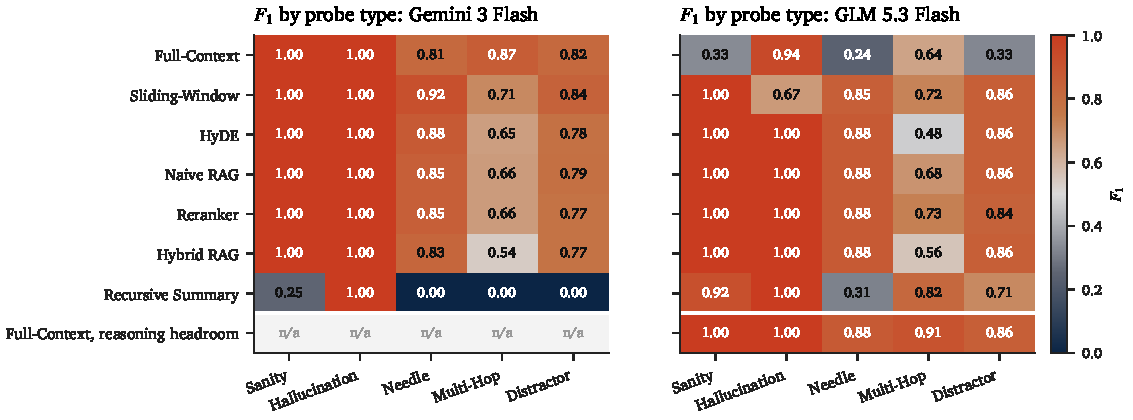
\includegraphics[width=0.95\textwidth]{probe_heatmap_cross_model.pdf}
\caption{Token $F_1$ by probe type on Gemini~3~Flash (left) and GLM~5.3~Flash (right), with the same row order. The bottom row adds the GLM~5.3~Flash Full-Context run with reasoning headroom. The probe-type axis is the lever a domain practitioner uses: a domain dominated by needle-style questions should prioritize the approaches with the highest needle scores.}
\label{fig:heatmap}
\end{figure*}

Fig.~\ref{fig:heatmap} reports per-probe-type $F_1$ on both generators, the figure that most directly supports the domain-aware recommendations in Section~\ref{sec:domain}.

Four observations hold across generators.
First, every retrieval strategy handles the sanity probes and refuses every hallucination probe.
Second, multi-hop is the probe type that best separates the retrieval strategies on both models (spreads of $0.54$ to $0.66$ and $0.48$ to $0.73$), Hybrid RAG is among the weakest retrieval strategies on it ($0.54$ and $0.56$), and Full-Context is the strongest strategy overall on it ($0.87$ on Gemini~3~Flash and $0.91$ on GLM~5.3~Flash with headroom).
Third, the retrieval strategies' needle scores are nearly identical across models ($0.83$ to $0.88$), while their distractor scores are somewhat higher on GLM~5.3~Flash ($0.84$ to $0.86$ against $0.77$ to $0.79$).
Fourth, Recursive Summary is weak on needle probes on both generators ($0.00$ and $0.31$), the probe type whose answers are exactly the specific identifiers that summaries compress away.

\subsection{Cost and Quality}

\begin{figure*}[!t]
\centering
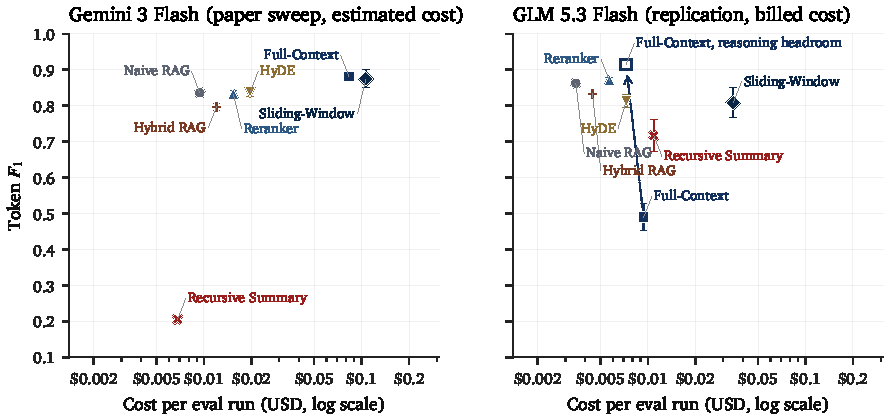
\includegraphics[width=0.95\textwidth]{pareto_cross_model.pdf}
\caption{Cost per full eval run (log scale) against token $F_1$ on each generator; error bars are seed standard deviations. Gemini~3~Flash costs are ledger estimates and GLM~5.3~Flash costs are billed amounts. Points that would coincide are nudged slightly apart horizontally for legibility; exact costs are in Tables~\ref{tab:headline} and~\ref{tab:crossmodel}. The dashed arrow marks the GLM~5.3~Flash Full-Context run with reasoning headroom.}
\label{fig:pareto}
\end{figure*}

Fig.~\ref{fig:pareto} maps the approaches onto the cost-quality plane for both generators.
On Gemini~3~Flash the four retrieval approaches sit at nearly identical cost ($\approx \$0.012$ per run); Full-Context and Sliding-Window cost approximately $7\times$ more for a $\Delta F_1 \approx 0.04$ premium.
On GLM~5.3~Flash the same retrieval cluster appears at lower billed cost ($\$0.004$ to $\$0.007$), and Full-Context with reasoning headroom reaches the top of the quality axis at comparable cost, because the long prompt is billed at a low input price.
Across all seven strategies a GLM~5.3~Flash run cost roughly one third of the estimated Gemini~3~Flash run; because one figure is billed and the other estimated, the ratio is indicative only.
The framework's cost ledger regenerates this plot for any generator the practitioner cares about.

\subsection{Seed Variance and Honesty}
\label{sec:variance}

\begin{figure}[!t]
\centering
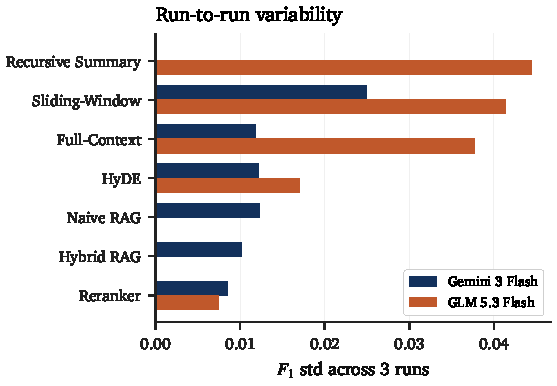
\includegraphics[width=0.92\columnwidth]{seed_variance.pdf}
\caption{$F_1$ standard deviation across three seeds on both generators. Multi-step pipelines (Sliding-Window, Recursive Summary) accumulate variance through their intermediate generations; single-call retrieval approaches are nearly deterministic.}
\label{fig:variance}
\end{figure}

\begin{figure}[!t]
\centering
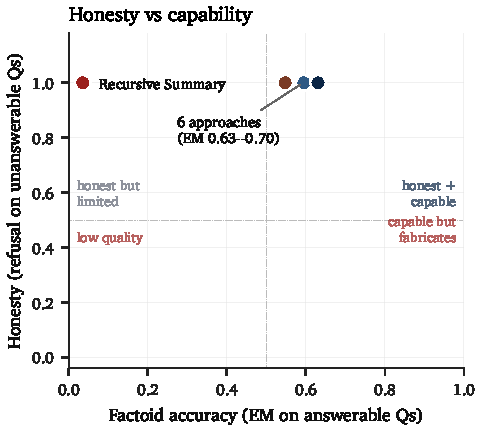
\includegraphics[width=0.95\columnwidth]{honesty.pdf}
\caption{Factoid accuracy (EM on answerable probes) and refusal accuracy (on unanswerable probes) for each approach, with one marker per generator on each row. Retrieval strategies refuse every unanswerable probe on both generators.}
\label{fig:honesty}
\end{figure}

Fig.~\ref{fig:variance} shows that single-call retrieval approaches are close to deterministic at $T = 0.3$ on both generators (Naive and Hybrid RAG have zero seed variance on GLM~5.3~Flash), while multi-step pipelines accumulate variance: Sliding-Window reaches $\sigma_{F_1} = 0.025$ on Gemini~3~Flash and $0.041$ on GLM~5.3~Flash, and Recursive Summary $0.044$ on GLM~5.3~Flash.
Fig.~\ref{fig:honesty} separates correctness into factoid recall and refusal accuracy.
All four retrieval strategies and Recursive Summary refuse every unanswerable probe on both generators; Sliding-Window refuses only two thirds of them on GLM~5.3~Flash, and the low-headroom Full-Context run slightly fewer than all.

\section{Domain-Aware Recommendations}
\label{sec:domain}

The probe-type breakdown in Fig.~\ref{fig:heatmap} provides the lever for translating these results into per-domain guidance.
Real-world domains differ primarily in the \emph{mix} of probe types their users issue.
We connect each major application domain to the probe distribution we believe characterizes it, anchored where possible to published evidence, and recommend the framework approach we expect to perform best.
Because the retrieval strategies behaved almost identically on both generators, these recommendations are not tied to one model, but they remain starting points; the framework's explicit invitation is that each domain practitioner replicate the evaluation on their own data and generator.

\paragraph{Medical question answering} is dominated by needle-style retrieval (specific drug names, dosages, ICD codes, contraindications) and by an unforgiving honesty requirement: a fabricated dose can harm a patient.
MedRAG~\cite{xiong2024medrag} reports that retriever choice substantially changes accuracy across the MIRAGE benchmark.
In our case study the retrieval strategies kept perfect refusal on both generators, and cross-encoder reranking was the strongest retrieval strategy overall on GLM~5.3~Flash and statistically tied on Gemini~3~Flash.
\textbf{Recommendation:} Cross-Encoder Reranker as the default; Full-Context when the medical record fits in the prompt and quality is paramount, with reasoning headroom for generators that reason.
\textbf{Avoid:} Recursive Summarization, which loses the numerical specifics medical answers require on both generators.

\paragraph{Legal retrieval and citation tasks} demand verbatim recall of statutes and precedents, multi-hop reasoning across clauses, and resistance to surface-similar distractors (e.g., a clause from a different statute).
LegalBench~\cite{guha2023legalbench} and its RAG extension~\cite{pipitone2024legalbenchrag} highlight retrieval as the primary failure mode in this domain.
Hybrid RAG was among the weakest multi-hop retrieval strategies on both generators, consistent with BM25's lexical bias being misled by surface-form similarity, while Full-Context led on multi-hop on both (on GLM~5.3~Flash once given reasoning headroom).
\textbf{Recommendation:} Full-Context for analyses within a single statute or contract; Cross-Encoder Reranker when the corpus is larger than the window.
\textbf{Caveat:} legal practitioners should add quotation faithfulness as a probe type beyond the five we use, because legal answers are evaluated as much on the cited passage as on the answer span.

\paragraph{Educational and tutoring use cases} value pedagogical explanation over verbatim extraction; multi-hop reasoning across textbook chapters is common, and the cost per response matters because student traffic is high-volume.
\textbf{Recommendation:} Naive Vector RAG or Cross-Encoder Reranker for cost-bounded student-facing deployments.
Recursive Summary may be acceptable here, because educational answers are often synthetic explanations rather than verbatim facts; its multi-hop score on GLM~5.3~Flash ($0.82$) suggests that with a capable summarizer it can serve synthesis-heavy questions, and this is one of the few domains in which summarization's information loss is tolerable.
\textbf{Caveat:} domain practitioners should add a ``pedagogical clarity'' probe type and a rubric-based evaluator beyond pure F$_1$.

\paragraph{Code understanding and software documentation} differs structurally from natural-language domains: chunks are not sentences but functions, classes, or commit blocks, and dense embeddings trained on prose under-represent symbol-level identity.
\textbf{Recommendation:} Hybrid RAG, weighting BM25 more heavily than in the case-study configuration so that exact-symbol matches are not diluted by dense-vector approximation.
The framework's chunker and tokenizer are configurable; an AST-aware chunker is a natural community contribution.

\paragraph{Finance and regulatory filings} share medical's needle-and-honesty profile (specific numbers, dates, percentages) with legal's multi-hop profile (cross-document reasoning across filings).
\textbf{Recommendation:} Cross-Encoder Reranker plus a tightened answer-formatting prompt to discipline numeric output; Full-Context when a single 10-K fits the window.
\textbf{Avoid:} Recursive Summary; specific financial figures are exactly the entities summarization compresses away, and needle recall stayed low on both generators.

\paragraph{High-stakes general QA over a fixed knowledge base} (internal wiki, FAQ bank, single-product handbook) typically has a corpus that already fits in modern context windows.
\textbf{Recommendation:} Full-Context Injection unless cost is the binding constraint, provisioning reasoning headroom for generators that reason; Cross-Encoder Reranker otherwise.

Across all six domains the consistent advice is to \emph{measure} on user-supplied data using the framework rather than rely on the case-study point estimates; the per-probe heatmap (Fig.~\ref{fig:heatmap}) and the cost-quality chart (Fig.~\ref{fig:pareto}) are the most directly transferable artifacts.

\section{Discussion}
\label{sec:discussion}

Six findings are supported by the data and inform framework users.

\paragraph{F1.~The pipeline matters more than the generator.}
For the four retrieval strategies, switching between a proprietary and an open-weights flash-tier generator moved $F_1$ by at most $3.8$ points, within the confidence intervals, while switching strategy on a single generator moved it by up to $67.5$ points.
For a given corpus and question mix, choosing and configuring the right pipeline is therefore the larger decision; the generator can be chosen on cost, latency, openness, or deployment constraints, and then verified with a replay rather than rediscovered from scratch.
This finding is bounded by our two generators and one corpus, and the framework is designed to test it on others.

\paragraph{F2.~Non-retrieval dominates at sub-window scale, given headroom.}
At the 8K-token regime tested here, placing the corpus in the prompt gave the highest $F_1$ on both generators.
The gap to the retrieval cluster is small ($\Delta F_1 \approx 0.04$) but consistent.
For generators that always reason, the advantage appears only when the reasoning budget is provisioned separately from the answer budget (Section~\ref{sec:headroom}); under a tight token limit the same strategy became the worst.
Practitioners whose corpus fits in the context window should treat Full-Context as the strong default and check the reasoning settings of their model.

\paragraph{F3.~Summarization loss is structural in kind, model-dependent in size.}
Recursive Summary's needle recall was poor on both generators ($0.00$ and $0.31$), confirming that question-agnostic summaries drop the specific identifiers factoid questions ask about.
Its overall $F_1$, however, ranged from $0.206$ to $0.717$, so a capable summarizer recovers much of the multi-hop and distractor performance.
Summarization should be avoided as a retrieval substitute for fact lookup, but it is model-sensitive enough that synthesis-heavy use cases should measure it rather than rule it out.

\paragraph{F4.~Refusal-prompt honesty transfers across retrieval pipelines.}
The strict-refusal instruction yielded $1.000$ refusal accuracy for all four retrieval strategies on both generators.
Production honesty for single-call retrieval pipelines can therefore be specified at the prompt level.
Multi-step pipelines are less robust: Sliding-Window's refusal accuracy fell to $0.667$ on GLM~5.3~Flash, so honesty should be re-measured whenever intermediate model outputs feed later steps.

\paragraph{F5.~Exact Match underestimates correctness and depends on formatting.}
On Gemini~3~Flash, EM stays near $0.667$ across six approaches whose $F_1$ spans $0.797$ to $0.881$; on GLM~5.3~Flash, many misses were formatting (``Seven years'' for the gold answer ``7 years'').
Because answer style varies by generator, frameworks evaluating short-factoid QA across models should report $F_1$ alongside EM and treat EM cautiously.

\paragraph{F6.~Multi-step pipelines require multi-seed evaluation.}
Sliding-Window and Recursive Summary show the largest seed variance on both generators, up to $\sigma_{F_1} = 0.044$, several times that of single-call retrieval approaches.
Single-seed reports of multi-step pipelines can misstate performance by several percentage points.

Which strategy to use remains a decision that depends on the corpus, the question mix, the cost envelope, and the generator.
The framework and the probe-level evidence in this paper are designed to make that decision cheap to take and easy to verify.

\section{Extension Points and Open Questions}
\label{sec:limits}

The framework is designed to be extended rather than treated as a closed result.
The case study reported here makes a deliberate set of choices that the framework explicitly invites users to revisit.

\paragraph{Corpus scale.}
The 8K-token corpus is small relative to many production deployments; we expect RAG approaches to reclaim their advantage once the corpus exceeds the context window.
Locating the crossover point on a user's own corpus is, by construction, a primary use case for the framework.

\paragraph{Sample size.}
$N = 34$ probes is small.
With Holm correction across 21 pairwise tests, only large deficits are statistically distinguishable on either generator.
Domain practitioners are encouraged to scale the probe set substantially (typical targets are $N \geq 200$) to resolve smaller differences; the framework imposes no upper bound on probe-set size.

\paragraph{Two generators, one corpus.}
The case study covers two flash-tier generators, one proprietary and one open-weights.
Transfer of the retrieval pipelines may not hold for much smaller models, models with weaker long-context attention, or very different answer styles.
Because the studio can replay the case study on any OpenRouter model, extending the comparison to frontier-scale, small, and locally hosted open-weight families~\cite{touvron2023llama} is a configuration change, and we particularly invite such replications.

\paragraph{Reasoning settings.}
Generators that reason introduce reasoning effort and token limits as additional experimental variables.
We report the settings used for every run; a systematic sweep of reasoning effort against strategy and corpus length is a natural next study.

\paragraph{Deferred approaches.}
Several retrieval techniques known in the literature are not yet implemented as reference approaches, including Self-RAG~\cite{asai2024selfrag}, GraphRAG~\cite{edge2024graphrag}, RAPTOR~\cite{sarthi2024raptor}, parent-child retrieval, multi-query retrieval, hierarchical RAG, contextual compression, prompt compression, explicit context caching, memory-augmented agents, and multi-agent memory architectures.
Each is a natural community contribution; the \texttt{Approach} protocol described in Section~\ref{sec:framework} is the contract a contributor satisfies.

\paragraph{Probe taxonomy.}
The five probe types we use cover much but not all of what production users care about.
Quotation faithfulness (legal), citation accuracy (academic), arithmetic robustness (finance), and pedagogical clarity (education) are obvious additions that the framework supports without code changes.

\paragraph{Temperature regime.}
The case study runs at $T = 0.3$, which is close to deterministic for short factoid answers.
Higher temperatures will increase seed variance and may affect honesty consistency; the framework runs the same sweep at any temperature.

\paragraph{Authorship bias in probe design.}
The probe set was authored by the same researchers who selected the approaches.
Domain replications by independent annotators are the natural way to remove this bias; the framework's evaluation files are plain JSONL and easy to audit.

The recurring theme is that the framework is intentionally a research scaffold rather than a closed result, and that its scientific value increases as the community uses it to validate and refine the case-study findings on real production corpora and other generators.

\section{Reproducibility and Open Source}
\label{sec:repro}

Every table and figure in this paper is regenerated from raw run artifacts by a single command (\texttt{make paper-ieee-regen}), which also exports the GLM~5.3~Flash replication from the studio's saved tests.
The complete framework, including the eval-set authoring guide, the seven reference approach implementations, the statistical-analysis CLI, the RAG Atlas studio, and the per-run artifacts, is publicly available as an open-source repository at \url{https://github.com/Singh-Gursahib/RAG-Approaches} under a permissive license.
Total LLM cost to reproduce the case study: USD~1.09 for the Gemini~3~Flash sweep and USD~0.26 for the GLM~5.3~Flash replication and its follow-ups.
The replication itself can be repeated on any other model from the studio's replay mode, and the cost of doing so is estimated before any call is made.

Contributions invited: additional reference approaches (especially structured retrievers), domain-specific evaluation corpora, alternative generator adapters, cross-model replications, and probe-type extensions.

\section{Conclusion}
\label{sec:conclusion}

We have presented an open-source, model-agnostic framework for the comparative evaluation of Retrieval-Augmented Generation strategies, demonstrated it on a hand-authored case study with two generators, and translated the probe-type breakdown into domain-aware recommendations.
The case study shows that retrieval pipelines behave almost identically on a proprietary and an open-weights generator, while the choice among strategies changes results by an order of magnitude more, and that long-context and summarization strategies need to be checked per model, including the reasoning settings of models that think before answering.
The framework's central thesis is that the right RAG for a given use case is an empirical question that depends on the corpus, the model, the cost envelope, and the probe distribution, and that it is best answered by direct measurement on the practitioner's own data with a tool that makes such measurement cheap, reproducible, and statistically honest.
The seven reference approaches we evaluate are a starting inventory, and the case-study findings are illustrative.
The framework, the probe-type taxonomy, the cost ledger, the studio, and the per-domain decision support are the durable contributions.

\section*{Acknowledgments}
We thank the maintainers of \texttt{sentence-transformers}, \texttt{ChromaDB}, \texttt{rank\_bm25}, and the BAAI FlagEmbedding project, whose freely available components made this framework feasible on a student budget.

\bibliographystyle{IEEEtran}
\bibliography{references}

\end{document}
